%%% Template originaly created by Karol Kozioł (mail@karol-koziol.net) and modified for ShareLaTeX use

\documentclass[11pt]{article}

\usepackage[T1]{fontenc}
\usepackage[utf8]{inputenc}
\usepackage{graphicx}
\usepackage{xcolor}
\usepackage{float}
\usepackage{tgtermes}
\usepackage{natbib}
%\usepackage[subnum]{cases}
\usepackage[super]{nth}
\bibpunct{(}{)}{;}{a}{}{,}
\usepackage{amsmath,amssymb}
\usepackage{enumerate}
\usepackage{multicol}
\usepackage{tikz}
\usepackage[amssymb]{SIunits}
\usepackage{rotating}
\usepackage{enumitem}
\usepackage{geometry}
\geometry{total={8.5in,11in},
left=1in,right=1in,%
bindingoffset=0mm, top=1in,bottom=1in}
\usepackage[super]{nth}
\usepackage{color}
\usepackage[
pdftitle={Homework 1}, 
pdfauthor={Jeremy Gibbs, University of Utah},
colorlinks=true,linkcolor=blue,urlcolor=blue,citecolor=blue,bookmarks=true,
bookmarksopenlevel=2]{hyperref}

\linespread{1.1}
\setlength{\parskip}{1em}
\setlength{\parindent}{0pt}
\newcommand{\linia}{\rule{\linewidth}{0.5pt}}

\makeatletter
\renewcommand{\maketitle}{
\begin{center}
\vspace{2ex}
{\huge \textsc{\@title}}
\vspace{1ex}
\\
\linia\\
ME EN 7960-003 \hfill Homework \#1 Solutions\hfill Due: September \nth{20}
\vspace{4ex}
\end{center}
}
\makeatother
%%%

% custom footers and headers
\usepackage{fancyhdr,lastpage}
\pagestyle{fancy}
\lhead{}
\chead{}
\rhead{}
%\lfoot{Assignment \textnumero{} 5}
\cfoot{}
\rfoot{Page \thepage~/~\pageref*{LastPage}}
\renewcommand{\headrulewidth}{0pt}
\renewcommand{\footrulewidth}{0pt}
%

%%%----------%%%----------%%%----------%%%----------%%%

\begin{document}

\title{Large-Eddy Simulation of Turbulent Flows}

\maketitle

%-- Question 1 --%
\vspace{-20pt}
\paragraph{1.) Pope Exercise 3.1}~\\\\
With $Q$ and $R$ being random variables, and $a$ and $b$, being constants use the following equation to verify that:
$$\langle Q(U) \rangle \equiv \int^{\infty}_{-\infty} Q(V) f(V) dV$$

\begin{enumerate}[label=(\alph*),topsep=-10pt]
	\item $\langle a \rangle = a$ and $\langle a Q \rangle = a \langle Q \rangle$\\	
	\textcolor{blue}{Using the above definition,
	$$\langle a \rangle = \int^{\infty}_{-\infty} a f(V) dV = a \int^{\infty}_{-\infty} f(V) dV$$
	We can invoke the normalization condition:
	$$\int^{\infty}_{-\infty} f(V) dV = 1$$
	Thus,$$\langle a \rangle = a \qquad \mbox{Rule 1}$$ $$\mbox{Similarly,}\qquad  \langle aQ \rangle = \int^{\infty}_{-\infty} a Q(V) f(V) dV = a \int^{\infty}_{-\infty} Q(V) f(V) dV = a\langle Q \rangle\qquad \mbox{Rule 2}$$
	}
	\item $\langle Q+R \rangle = \langle Q \rangle + \langle R \rangle$ and $\langle \langle Q \rangle \rangle = \langle Q \rangle$
	\textcolor{blue}{
	$$\langle Q+R \rangle = \int^{\infty}_{-\infty} [Q(V) + R(V)]f(V)dV = \int^{\infty}_{-\infty} Q(V)f(V)dV + \int^{\infty}_{-\infty} R(V)f(V)dV = \langle Q \rangle + \langle R \rangle \qquad \mbox{Rule 3}$$}
	\item $\langle \langle Q \rangle \langle R \rangle \rangle = \langle Q \rangle \langle R \rangle$ and $\langle \langle Q \rangle R \rangle = \langle Q \rangle \langle R \rangle$\\
	\textcolor{blue}{Since $\langle Q \rangle$ and $\langle R \rangle$ are constants, we can simply invoke Rules 1 and 2 from above:
	\begin{align*}
	\langle \langle Q \rangle \langle R \rangle \rangle &= \langle Q \rangle \langle R \rangle\\
	\langle \langle Q \rangle R \rangle &= \langle Q \rangle \langle R \rangle \qquad \mbox{Rule 4}
	\end{align*}}
	\item $\langle q^{\prime} \rangle = 0$ and $\langle q^{\prime} \langle R \rangle \rangle = 0$, where $q^{\prime} = Q - \langle Q \rangle$\\
	\textcolor{blue}{Using Rule 3:
	$$\langle q^{\prime} \rangle = \langle Q - \langle Q\rangle \rangle = \langle Q + \langle -Q\rangle \rangle = \langle Q \rangle + \langle -Q\rangle = \langle Q \rangle - \langle Q\rangle = 0$$
	Using Rule 5, since $\langle R \rangle$ is a constant:
	$$\langle q^{\prime} \langle R \rangle \rangle = \langle q^{\prime}\rangle \langle R \rangle = 0\langle R \rangle=0$$}
\end{enumerate}
Note: it is acceptable to use a rule (make sure to refer to it) after you have proven it.


%-- Question 2 --%
\paragraph{2.) Pope Exercise 3.2}~\\\\
Let $Q$ be defined by $Q = a + bU$, where $U$ is a stationary random variable and $a$ and $b$ are constants. Show that:
\begin{enumerate}[label=(\alph*),topsep=-10pt]
	\item $\langle Q \rangle = a + b\langle U \rangle$
	
	\textcolor{blue}{Using the definition of the mean from problem 1,
	\begin{align*}
	\langle Q(U) \rangle &= \int^{\infty}_{-\infty} (a + bV) f(V) dV\\
	&= \int^{\infty}_{-\infty} a f(V) dV + \int^{\infty}_{-\infty} bV f(V) dV\\ 
	&= a\int^{\infty}_{-\infty}f(V) dV + b\int^{\infty}_{-\infty} V f(V) dV\\ 
	&= a + b\langle U \rangle
	\end{align*}}
	\item $\text{var}(Q) = b^2\ \text{var}(U)$
	\textcolor{blue}{
	\begin{align*}
	\text{var}(Q) &= \int^{\infty}_{-\infty} [Q(V) - \langle Q(V)\rangle]^2 f(v) dV\\
		&= \int^{\infty}_{-\infty} [a + bV - (a + b\langle U \rangle)]^2f(V)dV\\
		&= \int^{\infty}_{-\infty} b^2 (V - \langle U \rangle)^2 f(V)dV\\
		&= b^2 \text{var}(U)
	\end{align*}}
	\item $\text{sdev}(Q) = b\ \text{sdev}(U)$
	\textcolor{blue}{
	$$\text{sdev}(Q) = \sqrt{ \text{var}(Q)} = \sqrt{b^2\text{var}(U)} = b\sqrt{\text{var}(U)} = b\ \text{sdev}(U)$$}
	\item $\text{var}(U) = \langle U^2 \rangle - {\langle U \rangle}^2$
	\textcolor{blue}{
	\begin{align*}
	\text{var}(U) &= \int^{\infty}_{-\infty} (V - \langle U \rangle)^2f(V)dV\\
	&= \int^{\infty}_{-\infty}[V^2 f(V) - 2V\langle U \rangle f(V) + \langle U \rangle^2 f(V)]dV\\
	&= \int^{\infty}_{-\infty} V^2 f(V)dV -2 \int^{\infty}_{-\infty} V\langle U \rangle f(V) dV + \int^{\infty}_{-\infty} \langle U \rangle^2 f(V) dV\\
	&= \langle U^2 \rangle - 2\langle U \rangle^2  + \langle U \rangle^2\\
	&= \langle U^2 \rangle - \langle U \rangle^2
	\end{align*}}

\end{enumerate}

%-- Question 3 --%
\paragraph{3.) Probability and statistics}~\\\\
Using the data set \textit{v1obsdata.txt}, located at \href{http://gibbs.science/les/homework/v1obsdata.txt}{http://gibbs.science/les/homework/v1obsdata.txt} or on Canvas, calculate and plot (if required) the following:
\begin{enumerate}[label=(\alph*),topsep=-10pt]
	\item Calculate the probability density function (PDF) of $V_1$ and plot it using an appropriate bin size (your choice). Describe why you chose your bin size.
	\begin{figure}[H]
	\centering
	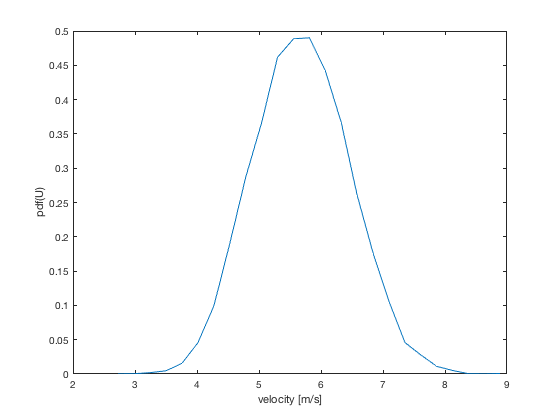
\includegraphics[width=0.9\textwidth]{pdf_25}
	\caption{PDF using 25 bins}
	\end{figure}
	\textcolor{blue}{You want to capture the PDF without introducing too much noise.}
	\item Calculate the first \textit{four} moments (mean, variance, skewness, and kurtosis) of the data and describe how each one is linked to the PDF you plotted in part (a). Note that you can calculate the moments from discrete estimates.\\\\
	\textcolor{blue}{Mean: 5.6873, Variance: 0.5964, Skew: 0.1058, Kurt: 2.8798\\\\
	The mean is the expected value in the PDF, the variance is how far the numbers are spread out from that mean, skewness is the asymmetry of the PDF (it is positive, which means that the PDF is skewed to the left), and kurtosis is the flatness of peak of the PDF (it is less than 3, so it is flatter than a Gaussian distribution)}
	\item Calculate and plot the autocorrelation function of the data. Comment on how well you can estimate the integral time scale from your plot.
	\begin{figure}[H]
	\centering
	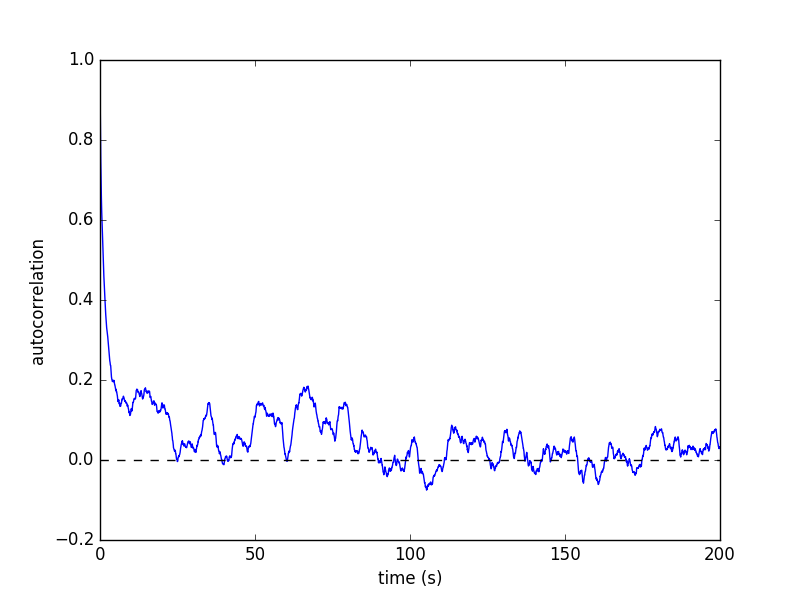
\includegraphics[width=0.9\textwidth]{autocorrelation}
	\end{figure}
\end{enumerate}


%-- Question 4 --%
\paragraph{4.) Power spectra}~\\\\
Using the data set \textit{v1simdata.txt}, located at \href{http://gibbs.science/les/homework/v1simdata.txt}{http://gibbs.science/les/homework/v1simdata.txt} or on Canvas, calculate and plot the 1D power spectral density as a function of wavenumber. Note that the data is a 2D horizontal slice from a 3D turbulence simulation. Calculate the power spectra in the streamwise ($x$) direction and then average the spectra over the spanwise direction so that your final estimation is:
$$\langle E_{11}(k_1) \rangle = \frac{1}{N_y} \sum_{j=1}^{N_y} \hat f_{k_1} \hat f^*_{k_1}$$
The data is saved in the file as ASCII text data with three columns. Column 1 is the $x$ streamwise position in meters, column 2 is the $y$ spanwise position in meters, and column 3 is the $V_1$ streamwise velocity in m/s. The 2D field has 256 points in each direction with $N_x = N_y = 256$. Make \textit{two} plots of the spectra (E11 vs k1): one with linear/linear scaling and a second with log/log scaling. Comment on any observations you can make about the shape of the spectra.
\begin{figure}[H]
	\centering
	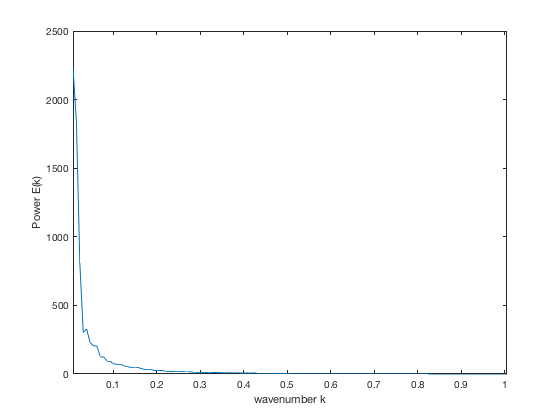
\includegraphics[width=0.8\textwidth]{spectra_linear}
	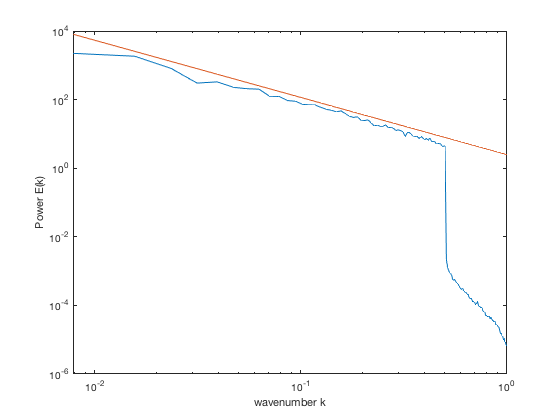
\includegraphics[width=0.8\textwidth]{spectra}
	\end{figure}
	\textcolor{blue}{The linear scale is hard to interpret. The log-log is much easier. The spectrum follows the -5/3 power law throughout the inertial subrange.}
\end{document}